%
% teil1.tex -- Beispiel-File für das Paper
%
% (c) 2020 Prof Dr Andreas Müller, Hochschule Rapperswil
%
\section{Fraktale
\label{ifs:section:teil1}}
\rhead{Problemstellung}
Bevor wir die IFS ansehen, schauen wir uns Fraktale genauer an.
Über die genaue Definition von Fraktalen sind sich die Mathematiker nicht einig. 
In diesem Kapitel orientieren wir uns an den Eigenschaften, welche Kenneth Falconer in seinem Buch {\em Fractal Geometry} \cite{ifs:fractal-geometry} beschreibt.
Von einem Fraktal $F$ können wir folgende Eigenschaften erwarten: 
\begin{enumerate}
	\item $F$ hat eine unendlich feine Struktur
	\item $F$ kann nicht mit der klassischen Geometrie beschrieben werden.
	\item Oftmals hat $F$ eine Form von Selbstähnlichkeit.
	Man spricht von einer selbstähnlichen Menge, wenn sich diese Menge überdecken lässt mit echten Teilmengen, die zur ganzen Menge ähnlich sind.
	\item Die `fraktale Dimension´ ist grösser als die topologische Dimension
	\item Viele Fraktale lassen sich auf eine simple Art definieren. Es genügen zum Beispiel nur wenige Funktionen, welche rekursiv ausgeführt werden, um ein Fraktal zu definieren.  
\end{enumerate}
\subsection{Koch Kurve
	\label{ifs:subsection:lilkoch}}
Diese Eigenschaften möchten wir nun am Beispiel der Koch Kurve näher anschauen.
In Abbildung \ref{ifs:kochkurve8} sehen wir die Koch Kurve. Sie besteht aus lauter kleineren Kopien von sich selbst. 
Der Konstruktionsvorgang ist in Abbildung \ref{ifs:kochconst} dargestellt.
Gestartet wird mit einer einzelnen Strecke der Länge $a$.
Diese wird in ersten Schritt durch vier gleich langen Streckenabschnitte der Länge $\frac{a}{3}$ ersetzt.
In \ref{ifs:kochconstb} ist die Anordnung dieser vier Streckenabschnitte ersichtlich. 
Dieser Schritt wird nun für jeden der resultierten Streckenabschnitten wiederholt.
Die Kurve besteht also aus vier kleineren Kopien der ganzen Kurve, was auch unter Selbstähnlichkeit bekannt ist.


\begin{figure}
	\centering
	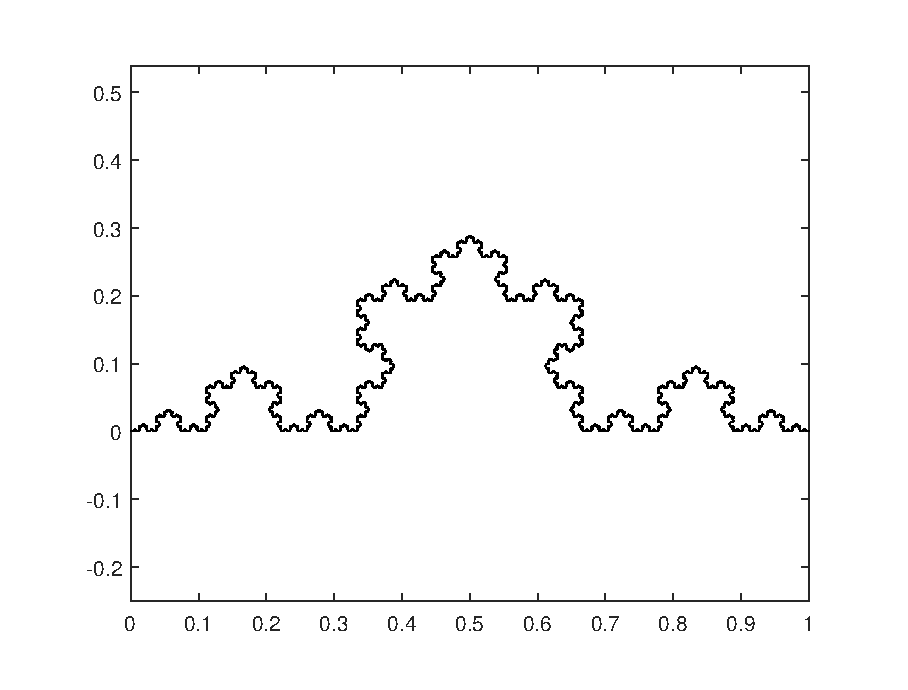
\includegraphics{papers/ifs/images/koch8}
	\caption{Koch Kurve}
	\label{ifs:kochkurve8}
\end{figure}

\begin{figure}
	\centering
	\subfigure[]{
		\label{ifs:kochconsta}
		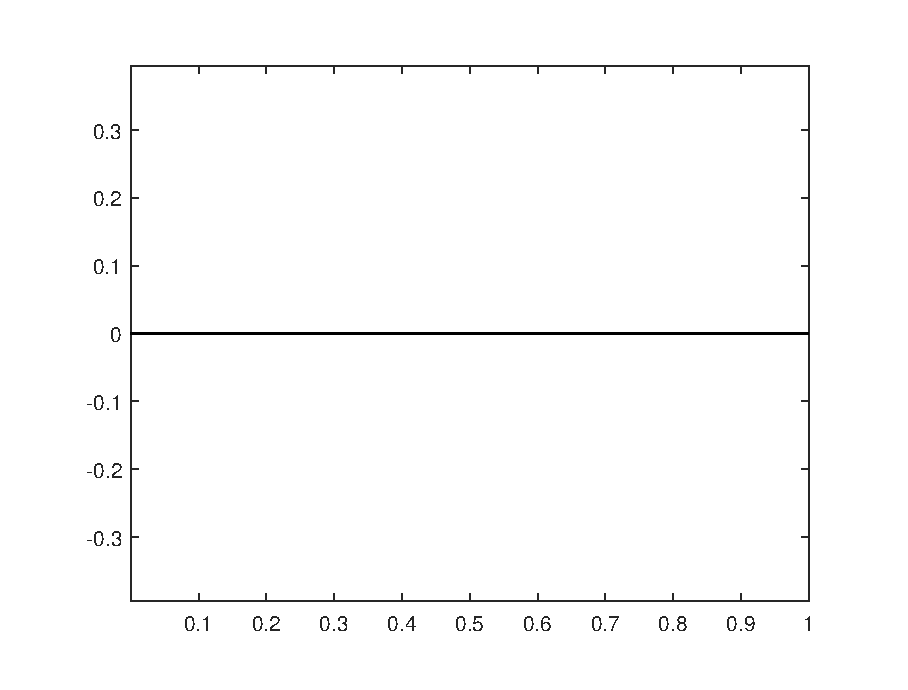
\includegraphics[width=0.32\textwidth]{papers/ifs/images/koch0}}
	\subfigure[]{
		\label{ifs:kochconstb}
		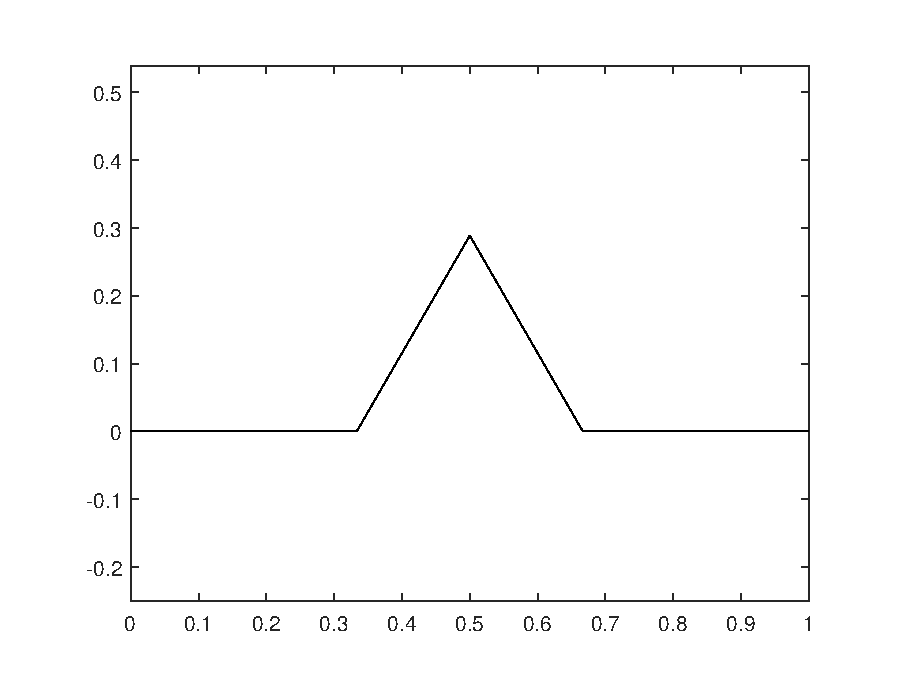
\includegraphics[width=0.32\textwidth]{papers/ifs/images/koch1}} 
	\subfigure[]{
		\label{kochconstc}
		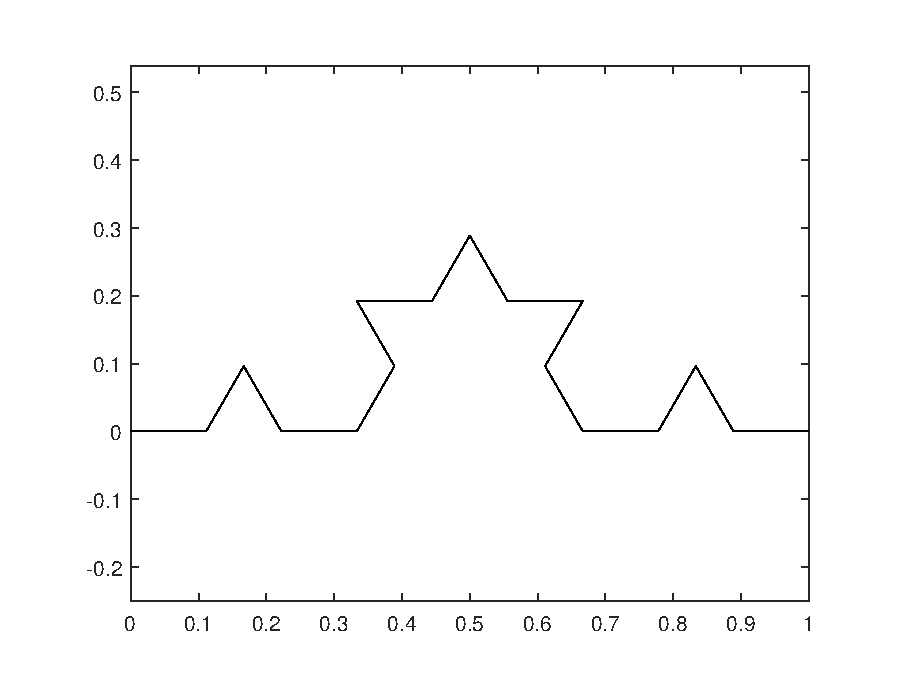
\includegraphics[width=0.32\textwidth]{papers/ifs/images/koch2}}
	\caption{(a) Start (b) 1. Iteration (c) 2. Iteration}
	\label{ifs:kochconst}
\end{figure}

Die resultierende Kurve hat ein paar interessante Eigenschaften.
Die Länge der Kurve der jeweiligen Iteration lässt sich mit 
\begin{align*}
	l_0 = a ,\quad l_1 = a  \frac{4}{3} ,\quad l_2 = a  \left( \frac{4}{3}\right)^2 , \quad \cdots , \quad
	l_n = a \cdot \left( \frac{4}{3}\right)^n \quad
	\Rightarrow \quad
	\lim_{n\to\infty} a  \left( \frac{4}{3}\right)^n = \infty
\end{align*}
berechnen.
In jedem Schritt wird die Länge um den Faktor $\frac{4}{3}$ verlängert. Daraus resultiert, dass die Länge gegen $\infty$ divergiert. 


Die Fläche der Kurve lässt sich folgendermassen berechnen
\begin{align*}
	A_0 &= 0 \\
	A_1 &= \left( \frac{a}{3}\right)^2 \frac{\sqrt{3}}{4} = a^2 \frac{\sqrt{3}}{36}\\
	A_2 &= A_1 + 4\left( \frac{a}{3^2}\right)^2 \frac{\sqrt{3}}{4} = A_1 + \frac{4}{9} A_1 \\ 
	A_3 &= A_1 + A_2 + 4^2 \left( \frac{a}{3^2}\right)^2 \frac{\sqrt{3}}{4} = A_1 + \frac{4}{9} A_1 + \left( \frac{4}{9}\right)^2 A_1.
\end{align*}
Wir sehen, dass mit jedem Schritt die neu dazugekommene Fläche um $\frac{4}{9}$ kleiner ist.
Die Gesamtfläche ist daher gegeben durch die konvergierende geometrische Reihe,
\begin{align*}
	A_n = A_1 \sum_{i = 0}^{n-1} \left( \frac{4}{9}\right)^n =  a^2 \frac{\sqrt{3}}{36} \sum_{i = 0}^{n-1} \left( \frac{4}{9}\right)^n \\
\end{align*}
mit dem Grenzwert
\begin{align*}
	\lim_{n\to\infty} a^2 \frac{\sqrt{3}}{36} \sum_{i = 0}^{n-1} \left( \frac{4}{9}\right)^n = \frac{\sqrt{3}}{20} a^2. 
\end{align*}
Wie wir sehen ist die Koch-Kurve ein Objekt mit endlicher Fläche, aber unendlichem Umfang.


Zu guter Letzt bestimmen wir die Dimension der Kurve. 
Es gibt viele verschiedene Methoden die Dimension zu definieren. Diese können dann auch unterschiedliche Resultate liefern.
Vor allem im Zusammenhang mit Fraktalen findet man in der Literatur unterschiedliche Arten.
Da die Kochsche Kurve selbstähnlich ist, ist die Ähnlichkeits-Dimension \cite{ifs:fractal-geometry} die angemessene Messzahl für die Dimension.
Die Ähnlichkeits-Dimension $D$ ist das Verhältnis der Logarithmen der Anzahl Kopien $N$ des Originales und deren Skalierungsfaktor $\epsilon$
  
\begin{align*}
	D = - \frac{\log N}{\log \epsilon }.
\end{align*}
Die Ähnlichkeits-Dimension stimmt für viele gewöhnliche Geometrische Objekte mit der intuitiven Vorstellung von Dimension überein.
Zum Beispiel besteht ein Dreieck aus $N = 4$ Kopien mit halber ($\epsilon = 1/2$) Kantenlänge $l$, Abbildung \ref{ifs:trinagle}.
Somit hat das Dreieck die Dimension $D = 2$.
Die Koch Kurve besteht aus $N = 4$ Kopien mit Kantenlänge $\epsilon =l \cdot 1/3$.
Ihre  Ähnlichkeits-Dimension ist somit
\begin{align*}
	D = - \frac{\log N }{\log \epsilon } = - \frac{\log 4 }{\log 1/3 } \approx 1.2619.
\end{align*}
Wie wir nun sehen besitzt die Koch-Kurve alle oben beschriebenen Eigenschaften von Fraktalen. 
Dies muss jedoch nicht bei allen Fraktalen der Fall sein. Sonst wäre die Frage nach einer 'richtigen' Definition einfach zu beantworten.
\begin{figure}
	\centering
	\begin{tikzpicture}
		
		% draw the background
		\draw [line width=1.5pt, fill=gray!2] (0,0) -- (60:4) -- (4,0) -- cycle;
		
		\coordinate[label=left:$A$]  (A) at (0,0);
		\coordinate[label=right:$B$] (B) at (4,0);
		\coordinate[label=above:$C$] (C) at (2,3.464);
		
		\coordinate[label=below:$l$](c) at ($ (A)!.5!(B) $);
		\coordinate[label=left:$l$] (b) at ($ (A)!.5!(C) $);
		\coordinate[label=right:$l$](a) at ($ (B)!.5!(C) $);
		
		\coordinate[label=below:$l/2$](d) at ($ (b)!.5!(a)$);
		
		% the triangle
		\draw [line width=1.5pt] (A) -- (B) -- (C) -- cycle;
		\draw [line width=0.5pt] (a) -- (b);
		\draw [line width=0.5pt] (a) -- (c);
		\draw [line width=0.5pt] (c) -- (b);
		
	\end{tikzpicture}
	\caption{Selbstähnlichkeit eines gleichseitigen Dreiecks}
	\label{ifs:trinagle}
\end{figure}

